% Define block styles
{
\tikzstyle{data} = [rectangle,  text width=5.5em, text centered, rounded corners, minimum height=4em]

\tikzstyle{header1} = [rectangle,   text centered, font=\fontsize{20}{0}\selectfont]
\tikzstyle{header2} = [rectangle,   text centered, font=\fontsize{10}{0}\selectfont,text width=6em]

\tikzset{database/.style={cylinder,aspect=0.5,draw,rotate=90,path picture={
\draw (path picture bounding box.160) to[out=180,in=180] (path picture bounding
box.20);
\draw (path picture bounding box.200) to[out=180,in=180] (path picture bounding
box.340);
}}}

\tikzstyle{proc} = [rectangle, draw,  text width=5em, text centered, rounded corners=0.2cm, minimum height=2em]

\small
    
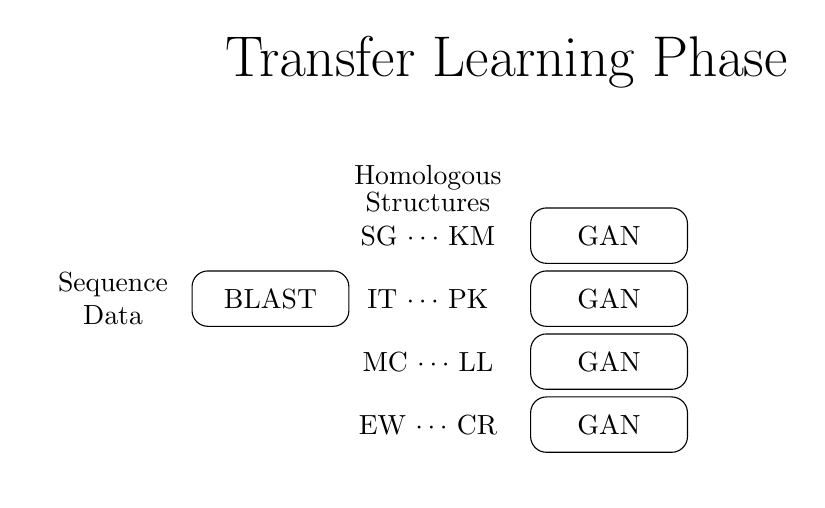
\begin{tikzpicture}[node distance = 2.5cm, auto]
    % Place nodes
    \node[header1] (tl_phase) at (0,2) {Transfer Learning Phase} ;
    \node [data] (sec) at (-5,-1){Sequence Data};
    \node [proc] (bls) at (-3,-1){BLAST};
    \node [data] (sec1) at (-1,-0.2){SG $\cdots$ KM};
    \node [data] (sec2) at (-1,-1){IT $\cdots$ PK};
    \node [data] (sec3) at (-1,-1.8){MC $\cdots$ LL};
    \node [data] (sec4) at (-1,-2.6){EW $\cdots$ CR};
    
    \node[header2] (hm_str) at (-1,0.4) {Homologous Structures} ;

    \node [proc] (gn1) at (1.3,-0.2){GAN};
    \node [proc] (gn2) at (1.3,-1){GAN};
    \node [proc] (gn3) at (1.3,-1.8){GAN};
    \node [proc] (gn4) at (1.3,-2.6){GAN};


%     \node [proc, right=0.5cm  of pdb] (pdb_smpl) {Structure Sampling};
%     \node [data,right=0.5cm  of pdb_smpl] (c_loc) {Candidate Locations};
%     \node [data,below=0.5cm  of c_loc] (lbls) {Labels};
%     \node [proc, right=0.5cm  of c_loc] (feat) {Feature Extraction};
%     \node [data,right=0.5cm  of feat] (ftrs) {Features};
%     \node [proc, right=0.5cm  of ftrs] (trng) {Training};
% 	\node [data,right=0.5cm  of trng] (cnns) {CNN classifier};

%     \draw (pdb) -- (pdb_smpl);
%     \draw[->] (pdb_smpl) -- (c_loc);

% %    \path [line] (identify) -- (evaluate);
%    \path [line] (evaluate) -- (decide);
%    \path [line] (decide) -| node [near start] {yes} (update);
%    \path [line] (update) |- (identify);
%    \path [line] (decide) -- node {no}(stop);
%    \path [line,dashed] (expert) -- (init);
%    \path [line,dashed] (system) -- (init);
%    \path [line,dashed] (system) |- (evaluate);
\end{tikzpicture}
}